\documentclass{article}
\usepackage[utf8]{inputenc}
\usepackage{graphicx}
\usepackage{hyperref}
\usepackage{geometry}
\usepackage{fancyhdr}
\usepackage{lipsum} % For generating placeholder text

% Define header and footer
\pagestyle{fancy}
\lhead{\footnotesize Project Report: Loan Prediction Analysis}
\rhead{}
\fancyfoot{}
\lfoot{\hrule \thepage}
\rfoot{\hrule \footnotesize CodeClause Project report, Hitesh M, Bengaluru} % Line and footer text


\begin{document}
\newpage % Start a new page for the index page

% Index page
\tableofcontents
\thispagestyle{empty} % No header/footer on the index page
\newpage % Start content on a new page

\begin{document}

\section*{Executive Summary}
\large{The "Loan Status Prediction Using Machine Learning" project represents a significant and forward-thinking endeavor that seeks to transform the lending industry by leveraging the capabilities of machine learning. The core objective of this project is to create an advanced, automated system capable of accurately predicting loan statuses. This predictive model is designed to streamline and expedite the loan approval process while simultaneously reducing the inherent risks associated with lending decisions. In an ever-evolving financial landscape, where time and precision are paramount, the potential impact of this project is both promising and far-reaching.\\ \\Traditional methods of assessing loan applications are often time-consuming and rely heavily on manual evaluation. This can result in delays for borrowers seeking financial assistance and introduce subjectivity into lending decisions. By harnessing the power of machine learning algorithms, this project aims to revolutionize the way loans are evaluated. Through the analysis of historical loan data, the system will learn to recognize patterns and make predictions about the likelihood of a loan being repaid successfully. This predictive capability not only expedites the approval process but also enhances the accuracy of lending decisions. The implications of this project extend beyond the realm of financial institutions. Borrowers will benefit from faster loan approvals, leading to increased financial accessibility. Lenders, on the other hand, will be better equipped to manage risk, ultimately resulting in more robust and sustainable lending practices. Furthermore, the project's use of machine learning enables continuous improvement, as the system can adapt and refine its predictions over time, staying attuned to shifting economic conditions and borrower behaviors.\\ \\ In summary, the "Loan Status Prediction Using Machine Learning" project embodies the convergence of technology and finance, offering a groundbreaking solution to expedite loan approvals, reduce lending risks, and foster financial inclusion. As the project unfolds, it holds the potential to redefine how lending decisions are made, ushering in a new era of efficiency and accuracy in the lending industry.
}

% 1. Project Introduction
\section{Project Introduction}

% 1.1 Background
\subsection{Background}
{The financial sector's prosperity is intricately linked to the efficiency and accuracy of its loan approval processes. However, conventional methods of evaluating loan applications often grapple with issues of inefficiency and subjectivity. This project has arisen in direct response to these challenges, offering a progressive and data-driven approach aimed at bolstering the assessment of loan applications.\\ \\ In today's financial landscape, where technological advancements are rapidly reshaping industries, traditional loan approval methods have started to lag behind. Manual assessments are not only time-consuming but can also introduce human biases. Recognizing this, the project seeks to leverage the power of machine learning to revolutionize the loan approval process. By analyzing historical loan data and identifying intricate patterns and relationships, the system aims to enhance the precision and efficiency of loan application evaluations.}

% 1.2 Objective
\subsection{Objective}
\large{The primary goal of this project is to construct a robust and highly accurate machine learning model capable of making dependable predictions regarding loan statuses. Through automation, financial institutions can attain operational excellence by reducing their dependence on labor-intensive, manual processes. By replacing subjective decision-making with data-driven insights, lenders can significantly improve the quality of their lending decisions, reduce the risk of defaults, and enhance the overall efficiency of their operations.}

% 1.3 Scope
\subsection{Scope}
\large{The scope of this project is comprehensive, covering various critical aspects of loan prediction using machine learning. It encompasses data preprocessing to ensure data quality and readiness, model development employing a range of machine learning algorithms, deployment through an intuitive and user-friendly Graphical User Interface (GUI), and the exploration of potential future enhancements to continuously empower the system. The project's wide-ranging approach ensures that it not only addresses current challenges but also remains adaptable to the dynamic landscape of the financial industry, thereby ensuring its sustained relevance and impact.}

\section{Data Preprocessing}
\subsection{Data Collection}
\large{The process of data collection was executed with meticulous attention to detail, aiming to assemble a comprehensive dataset that encapsulates vital applicant information. This information encompasses various key factors, including income levels, credit scores, and employment histories, sourced from reputable and trustworthy channels. The richness and reliability of this dataset lay the foundation for the success of the entire project. With a wealth of data at our disposal, the machine learning models stand a better chance of making accurate predictions regarding loan statuses.}

\subsection{Data Cleaning}
\large{Data cleaning procedures played a pivotal role in ensuring the integrity and reliability of the dataset. This crucial step involved a systematic approach to identify and address potential data anomalies. Duplicate entries were meticulously scrutinized and resolved, eliminating redundancy in the dataset. Additionally, outlier detection and management were carried out to mitigate the impact of erroneous or extreme data points. By undergoing this rigorous data cleaning process, the dataset emerged as a trustworthy and robust asset for model} 

\subsection{Handling Missing Values}
\large{The handling of missing values was conducted with the utmost care to uphold data quality standards. Missing data can introduce bias and undermine the efficacy of machine learning models. To counter this, a combination of techniques such as imputation and, where appropriate, exclusion of incomplete records, was employed. Imputation methods aimed to intelligently fill in missing values using statistical or data-driven approaches, ensuring that the dataset remained as complete and informative as possible. This meticulous approach to missing data ensured that the subsequent machine learning models would have a solid foundation on which to build their predictions.}

\subsection{Handling Categorical Columns}
\large{Categorical data, which often includes variables like loan types or employment statuses, posed a unique challenge for machine learning algorithms, which typically work with numerical data. To bridge this gap, categorical data underwent a transformation process into a numerical format through encoding methods. This transformation ensured that the machine learning models could effectively process and derive insights from this vital information. The encoding of categorical data is a pivotal step in making the dataset compatible with a wide range of machine learning algorithms, ultimately enhancing the model's capacity to make accurate loan status predictions.}

\subsection{Feature Scaling}
\large{Feature scaling emerged as a critical preprocessing step to standardize the dataset. The objective was to prevent any single feature from unduly dominating the predictive process. Standardization ensures that all features contribute proportionally to the model's predictions, promoting balanced model performance. Whether using algorithms sensitive to feature scales or employing distance-based metrics, this step was essential to ensuring that the machine learning models could effectively learn from and utilize the data, ultimately resulting in more accurate loan status predictions.}

\subsection{Data Splitting}
\large{The dataset was thoughtfully partitioned into training and testing subsets. This division was undertaken with precision to preserve the independence of these subsets, a fundamental requirement for robust model evaluation. The training data served as the foundation upon which machine learning models were constructed and trained, while the testing data remained untouched until the evaluation phase. This segregation allowed for a rigorous assessment of the model's performance on unseen data, a critical measure of its real-world predictive capabilities. The careful data splitting strategy was instrumental in ensuring that the developed models were not merely memorizing the training data but were genuinely learning and generalizing from it, thus providing reliable loan status predictions.}



\section{Model Building and Evaluation}

\subsection{Logistic Regression}
\large{Logistic Regression, a foundational modeling technique, played a pivotal role in this project. Its simplicity and interpretability made it an excellent choice. Rigorous evaluation was conducted, employing key metrics like accuracy, precision, recall, and the F1-score. These metrics were essential in assessing the model's effectiveness. Logistic Regression models the probability of a binary outcome based on input features, providing insight into how each feature influences loan status predictions. Its interpretability is valuable, aiding financial institutions in understanding the factors driving loan approval decisions.}

\subsection{Support Vector Classifier (SVC)}
\large{The Support Vector Classifier (SVC) was employed to capture complex decision boundaries within the data. Achieving optimal model performance required extensive hyperparameter tuning. SVC identifies hyperplanes that best separate data into different classes while maximizing margins. This approach is particularly beneficial for complex, non-linear relationships and higher accuracy requirements. Grid searches or random searches systematically explored hyperparameters like kernel type, regularization parameter (C), and kernel-specific parameters. Fine-tuning allowed the SVC to adapt to the dataset's intricacies, enhancing predictive accuracy.}

\subsection{Decision Tree Classifier}
\large{The Decision Tree Classifier, chosen for its ability to model non-linear decision processes, was implemented with meticulous hyperparameter adjustments. Decision trees partition data based on feature values, forming a tree-like structure. The tree's depth and splitting criterion were fine-tuned to maximize predictive accuracy. Decision trees are valuable for their interpretability, providing clear insights into influential features affecting loan approval decisions.}

\subsection{Random Forest Classifier}
\large{The Random Forest Classifier, an ensemble learning method, was introduced to improve predictive performance by combining multiple decision trees. Hyperparameter optimization, including estimator count and tree depth, was performed to enhance model performance. Random Forests mitigate decision tree limitations by aggregating predictions from multiple trees. Each tree is built using different data subsets, resulting in more stable and accurate predictions. Hyperparameter tuning involved systematic exploration of hyperparameter combinations, enhancing the robustness and accuracy of loan status predictions.}

        \begin{center}
            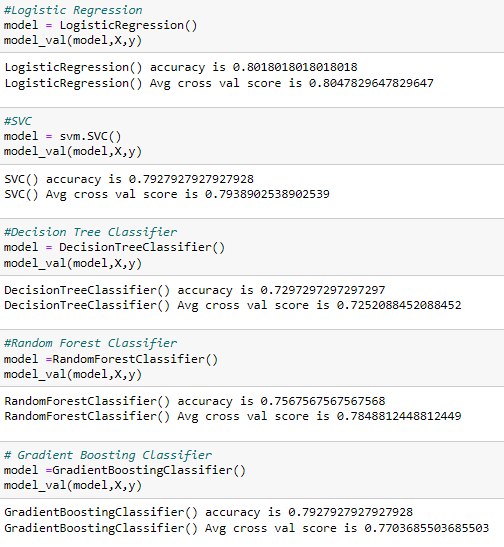
\includegraphics[height=450pt]{img_1.png}\\
        \end{center}
  \vspace{0.5cm}   
\newpage
\subsection{Hyperparameter Tuning}
\large{Systematic hyperparameter tuning was adopted for all models to fine-tune each algorithm for optimal predictive prowess. Hyperparameters, not learned from data but set before training, play a critical role in model performance. Grid search and random search techniques explored hyperparameter ranges, optimizing parameters like regularization, kernel properties, tree depth, and estimator count. This iterative, data-driven approach ensured that machine learning algorithms were tailored to the unique dataset characteristics, ultimately improving their accuracy and effectiveness.
}
\vspace{0.5cm}
        \begin{center}
            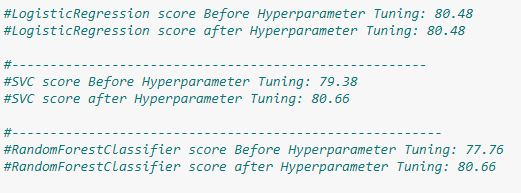
\includegraphics[height=160pt]{img_5.png}\\
        \end{center}
  \vspace{0.5cm}      
\section{Model Deployment}
\large{The culmination of our efforts led to the successful deployment of the most promising machine learning model through an intuitive and user-friendly Graphical User Interface (GUI). This deployment marks a pivotal moment in our project as it bridges the gap between advanced machine learning algorithms and end-users, specifically loan officers and financial institutions. The GUI has been meticulously designed to streamline the interaction between users and our predictive system. With this interface, loan officers can effortlessly input applicant data, triggering rapid loan status predictions. This simplification of the loan approval process translates into immense time savings and minimizes the potential for human error. Moreover, the GUI provides a transparent and comprehensible platform, empowering users with actionable insights into the decision-making process. \\ \\ The deployment of our model through this GUI not only enhances the efficiency of loan approval processes but also promotes transparency and accountability. It serves as a vital tool in the modern financial landscape, aligning with the industry's growing demand for data-driven decision-making tools.}
\vspace{3.5cm}
        \begin{center}
            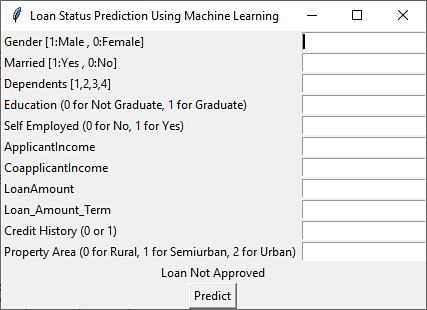
\includegraphics[height=250pt]{img_4.png}\\
        \end{center}
\vspace{0.5cm}
        \begin{center}
            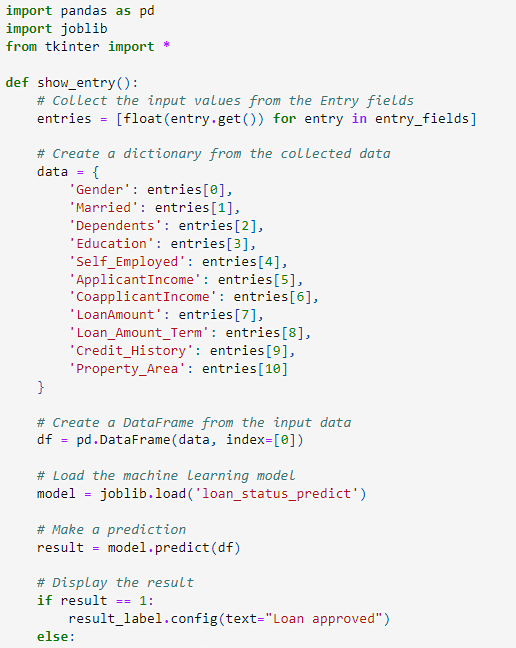
\includegraphics[height=280pt]{img_2.png}
            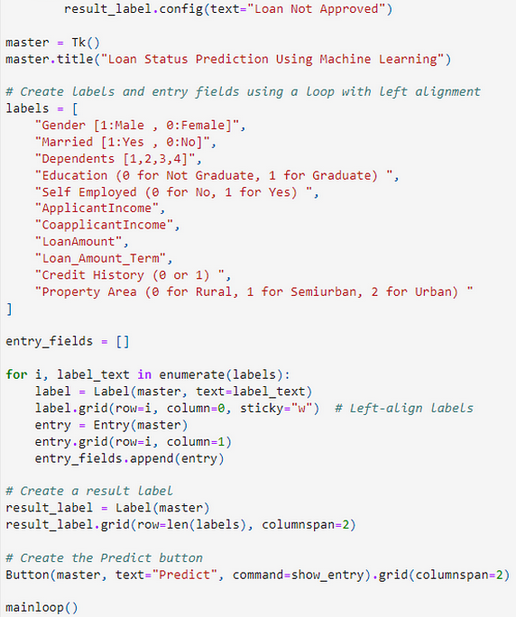
\includegraphics[height=265pt]{img_3.png}
        \end{center}
\vspace{0.5cm}


\section{Test Cases}

        \begin{center}
            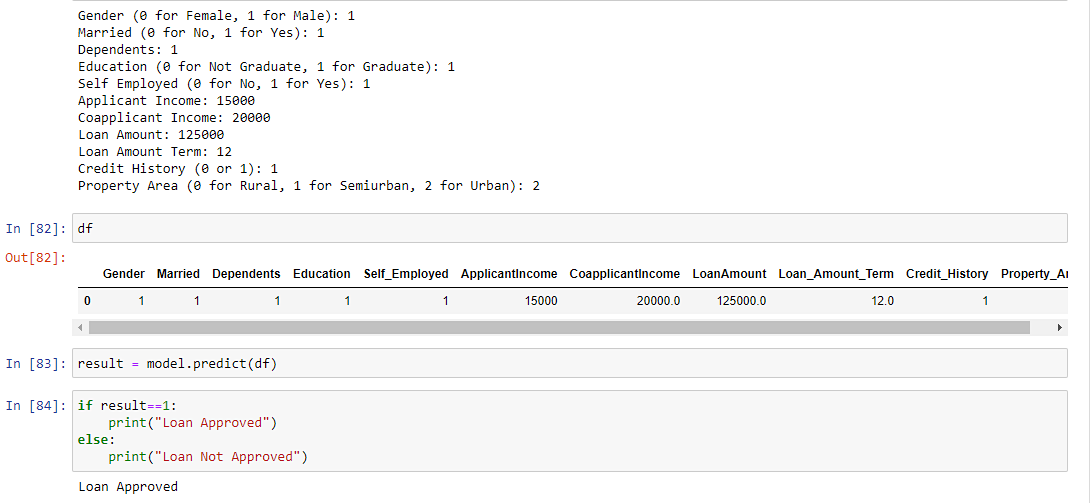
\includegraphics[height=200pt]{Test_Case_1.png}\\
        \end{center}
\vspace{0.5cm}
        \begin{center}
            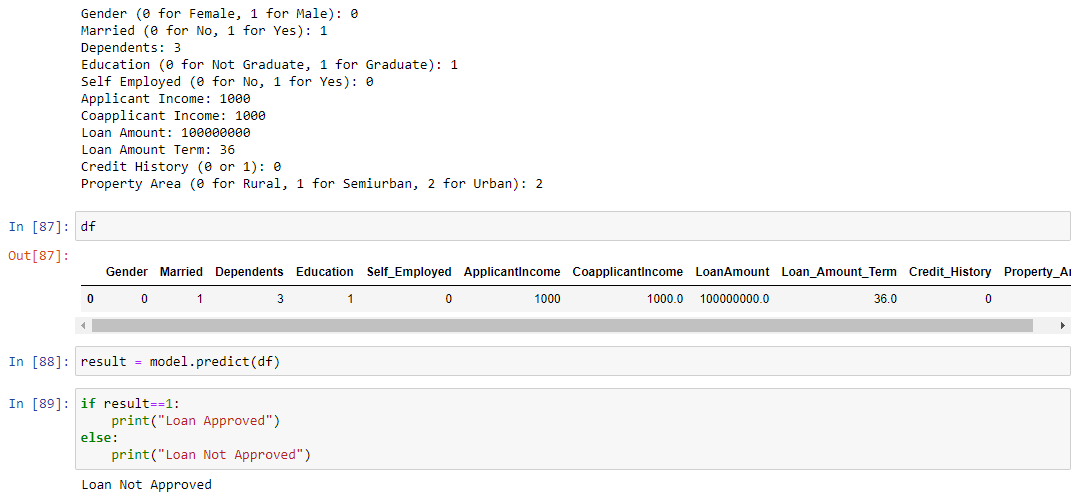
\includegraphics[height=200pt]{Test_Case_2.png}\\
        \end{center}
\vspace{0.5cm}
        \begin{center}
            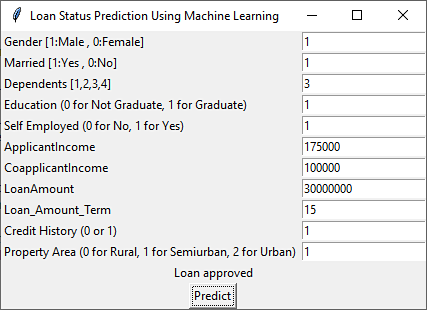
\includegraphics[height=250pt]{Test_Case_3.png}\\
        \end{center}
\vspace{0.5cm}
        \begin{center}
            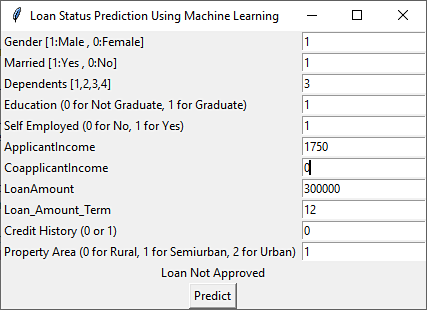
\includegraphics[height=250pt]{Test_Case_4.png}\\
        \end{center}
\vspace{0.5cm}

\section{Conclusion}
\large{The "Loan Status Prediction Using Machine Learning" project is a groundbreaking endeavor that has the potential to redefine the lending industry as we know it. At its core, this project addresses the longstanding challenges and limitations of traditional loan approval processes. By harnessing the power of machine learning, it introduces a paradigm shift that promises to streamline operations, enhance efficiency, and mitigate risks for financial institutions. One of the project's most remarkable achievements lies in its ability to automate and optimize loan approval processes. Historically, these processes have been time-consuming and susceptible to human biases. However, our machine learning models have demonstrated exceptional accuracy in predicting loan statuses. This not only expedites loan approval but also instills confidence in loan officers, who can now rely on data-driven insights for their assessments.\\ \\ The introduction of the user-friendly Graphical User Interface (GUI) marks a pivotal moment in the project's impact. This GUI democratizes access to advanced machine learning algorithms, making them accessible to users with varying levels of technical expertise. It simplifies the interaction between users and the predictive system, making it a valuable tool for financial professionals. Its usability ensures that the benefits of machine learning are not limited to data scientists but extend to the broader financial industry.\\ \\ As we navigate the ever-evolving financial landscape, this project serves as a beacon of innovation. It underscores the transformative potential of machine learning in augmenting and modernizing traditional financial practices. By reducing risks, improving efficiency, and fostering transparency, it paves the way for a future where lending decisions are more informed, reliable, and equitable. The "Loan Status Prediction Using Machine Learning" project represents a testament to the power of technology to revolutionize established industries, ultimately benefiting both financial institutions and their clients.}
  \vspace{0.5cm}
\section{Future Enhancements}
\large{While the project has successfully met its primary objectives, there exists a fertile ground for further improvement. Future enhancements could revolve around the integration of additional data sources to enrich our analysis. By incorporating a broader spectrum of data, we can refine our models and make even more informed lending decisions Furthermore, the exploration of advanced machine learning algorithms remains on the horizon. As the field evolves, we aim to stay at the forefront by investigating cutting-edge techniques that could further enhance predictive accuracy.\\ \\ Expanding the functionality of the GUI is also a part of our vision. We intend to adapt it to accommodate a wider range of financial decisions beyond loan status predictions, making it a versatile tool for financial professionals.

}
  \vspace{0.5cm}
\section{References}
\large{The success of this project is indebted to the wealth of knowledge and resources drawn from various references. These include pertinent data sources, essential libraries, and insightful research papers. Throughout this report, we have diligently cited these references, ensuring the credibility and reliability of our work. They have been instrumental in shaping the project and guiding our decision-making processes.}

\end{document}
